%%%%%%%%%%%%%%%%%%%%%%%%%%%%%%%%%%%%%%%%%%%%%%%%%%%%%%%%%%%%%%%%%%%%%%%%%%%%%%%%

\documentclass[a4paper, 10pt ]{article}     

% The following packages can be found on http:\\www.ctan.org
\usepackage{graphics} % for pdf, bitmapped graphics files
\usepackage{epsfig} % for postscript graphics files
\usepackage{mathptmx} % assumes new font selection scheme installed
\usepackage{times} % assumes new font selection scheme installed
\usepackage{amsmath} % assumes amsmath package installed
\usepackage{amssymb}  % assumes amsmath package installed
\usepackage[usenames]{color}
\usepackage[utf8]{inputenc} 

\title{\LARGE \bf
 Pré-manip Handibio
}


\author{Claire Dune, Cyril Joly}



\begin{document}
\maketitle
\thispagestyle{empty}
\pagestyle{empty}
%%%%%%%%%%%%%%%%%%%%%%%%%%%%%%%%%%%%%%%%%%%%%%%%%%%%%%%%%%%%%%%%%%%%%%%%%%%%%%%%

\section{Objectif de l'expérimentation}

L'objectif de cette expérimentation est triple : 
\begin{enumerate}
\item aquérir la posture lors de la marche avec et sans déambulateur pour pouvoir établir des comparaisons. 
\item aquérir des informations avec le déambulateur instrumenté.
\item prendre en main tous les systèmes d'acquisition pour les futures manips
\end{enumerate}

\section{Protocole}

Chaque sujet devra parcourir 5m en avant, en marchant tout droit. Sur ces 5m, au moins 3 m devraient être complétement couverts par la zone de travail des caméras. Les conditions expérimentales suivantes seront testées 5 fois pour chaque personnes : 

\begin{enumerate}
\item Marche sans déambulateur à allure normale.
\item Marche sans déambulateur à allure lente en trainant les pieds.
\item Marche avec déambulateur en s'appuyant sur le déambulateur a allure normale.
\item Marche avec déambulateur en s'appuyant sur le déambulateur et en trainant des pieds.
\end{enumerate}

\section{Matériel}

Dans cette manip, nous utiliserons les 6 caméras Qualysis ainsi qu'un déambulateur équipé de capteurs.

\subsection{Utilisation du Qualisys}

Pour cette expérience, il faut positionner les caméras de sorte à avoir une zone étalonnée qui couvre un chemin rectiligne de 3m de long permettant de voir à la fois les pieds et la tête du marcheur. \\

\subsection{Utilisation du logiciel}
Voici la marche à suivre pour utiliser le soft Qualisys.

\begin{enumerate}
\item positionner les 6 caméras approximativement pour couvrir la zone de travail
\item Brancher les caméras sur le secteur + les cables USB et ethernet
\item Configuration du réseau : Qualisys DHCP serveur (attention, réseau local à IP fixe)
\item Lancer le soft Qualisys track manager (indication 120Hz maxi)
\item Réglages $>$ Caméra $>$ Connection pour localiser les 6 caméras. Lorsque les 6 caméras sont localisées, on peut changer la fréquence d'acquisition. Pour la calibration, il faut une minute a 200 Hz, soit 12 000 frames.
\item File $>$ new ... pour créer la nouvelle manip
\item Calibration
\begin{enumerate}
\item fixer la duree de la calibration a une minute au moins pour une grande zone de travail.
\item lancer la calibration
\item pour que le résultat soit bon, il faut un résidu $r<1$
\item une fois la calibration faite, on peut afficher la zone calibrée pour vérifier la précision sur la zone de travail.
\end{enumerate}
\item Enregistrer la manip
\item Labéliser (touche MAJ+L)
\item On peut ensuite faire une création de modèle pour pouvoir le réutiliser pour les autres manips. (touche MAJ + B). Le menu s'appelle "AIM Generate Model"
\end{enumerate}


\subsubsection{Positionnement des marqueurs sur le sujet }

La figure \ref{fig:definitionQ} présente un modèle géométrique simplifié de l'homme avec les différents degrès de liberté de ses articulations.
Les figures \ref{fig:marqueursFace} et \ref{fig:marqueursDos} présentent  un positionnement des marqueurs respectivement sur une vue de face  et sur une vue de dos du sujet. Pour positionner les marqueurs, on se base sur les recommandation de la société international de biomécanique \cite{Wu02, Wu05}.
\begin{figure}
\includegraphics[width=0.7\columnwidth]{images/modeleHommeQ.eps}
\label{fig:definitionQ}
\caption{Représentation géométrique simplifiée du corps humain pour identifier les degrès de liberté.}
\end{figure}

\begin{figure}
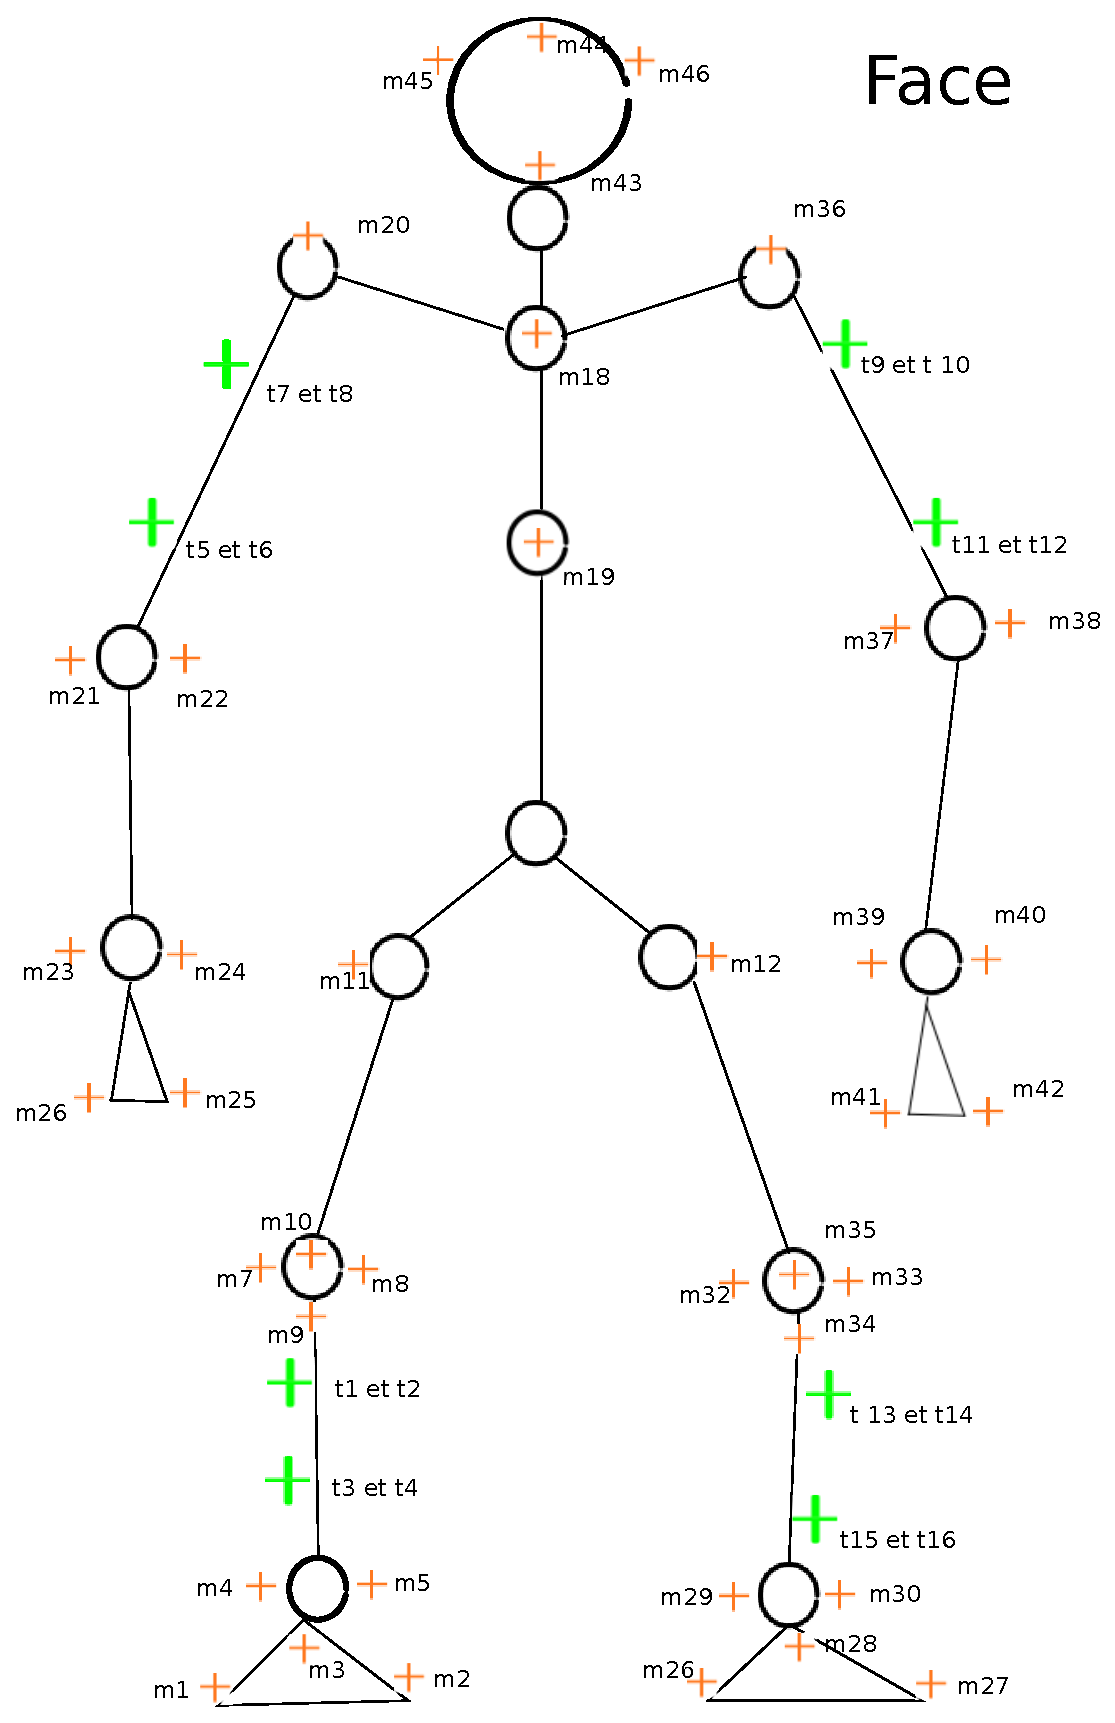
\includegraphics[width=0.7\columnwidth]{images/modeleHomme.eps}
\label{fig:marqueursFace}
\caption{Vue de face : positionnement des marqueurs. En orange, les marqueurs biomécaniques et en vert des marqueurs techniques.}
\end{figure}

\begin{figure}
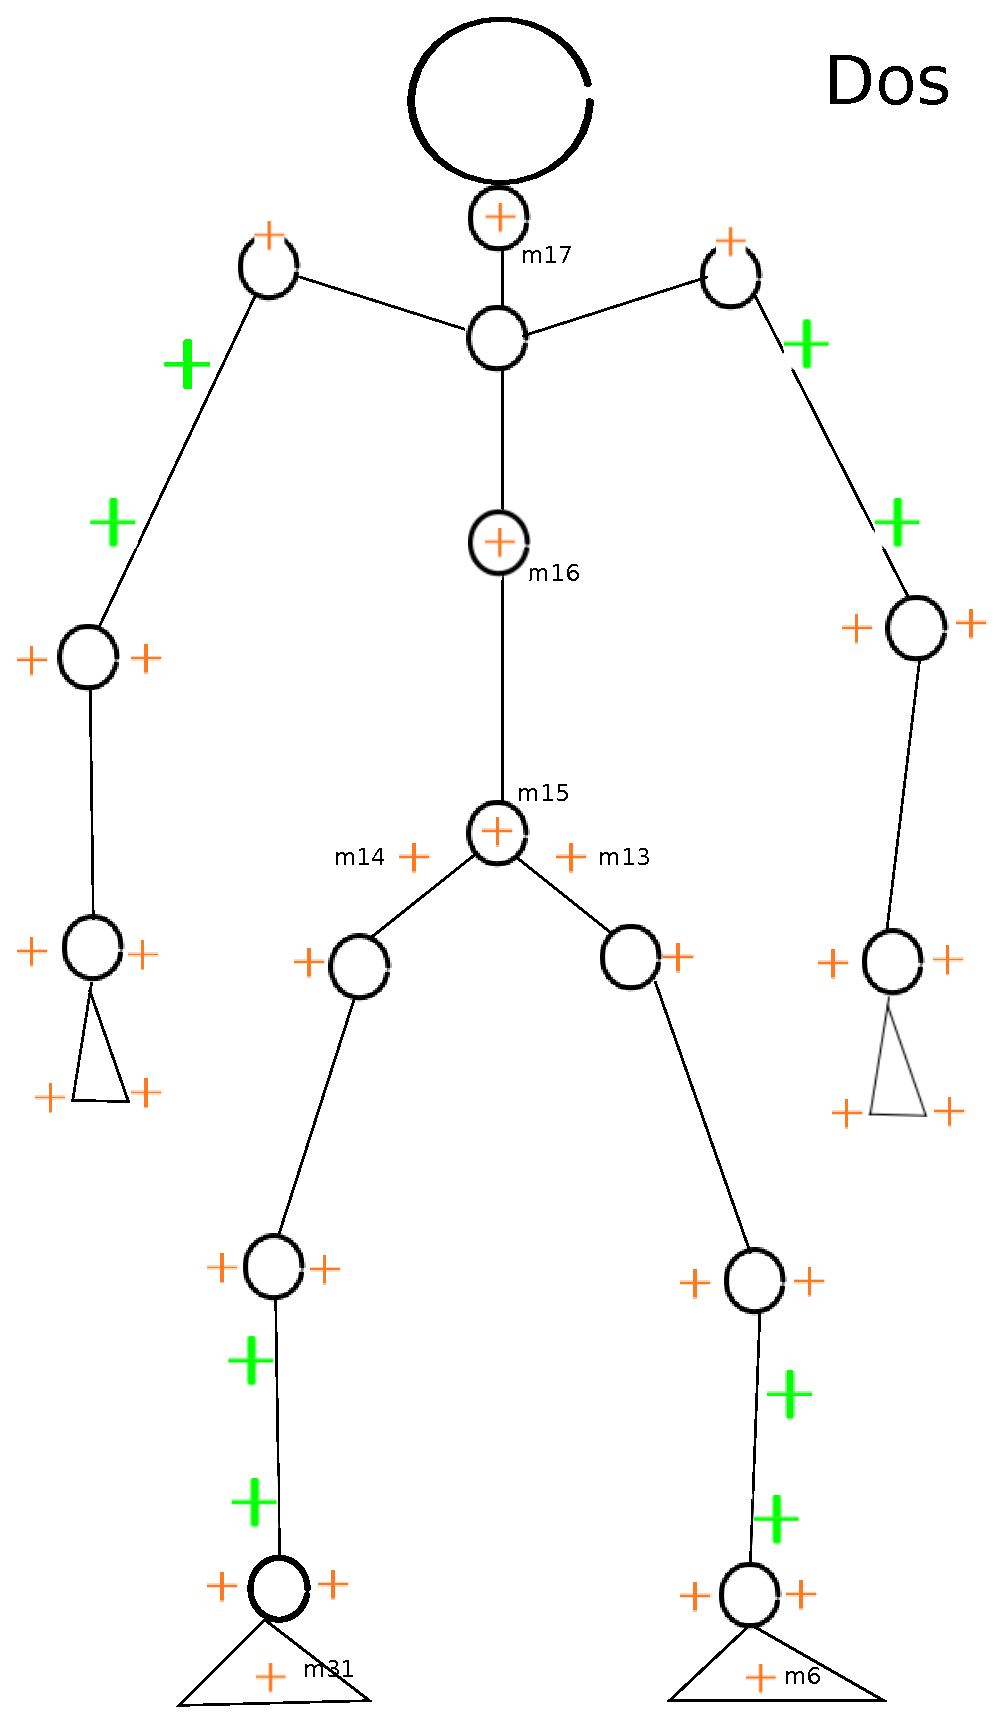
\includegraphics[width=0.7\columnwidth]{images/modeleHommeDos.eps}
\label{fig:marqueursDos}
\caption{Vue de dos : positionnement des marqueurs. En orange, les marqueurs biomécaniques et en vert des marqueurs techniques.}
\end{figure}

\begin{itemize}
\item Pied droit
\begin{itemize}
\item $m1$ et $m2$ (ajout) sur les phalanges métatarses mediales et latérales
\item $m3$ sur l'articulation du 3e métatarse (IM)
\item $m4$ et $m5$ respectivement sur le maleole latérale (LM) et médiale (MM)
\item $m6$ (ajout) sur le talon
\end{itemize}
\item Genou droit
\begin{itemize}
\item $m7$ (LC) la limite externe condyle tibial lateral
\item $m8$ (MC) la limite interne du condyle tibial médial
\item $m9$ (TT) sur la tuberosité tibiale
\item $m10$ (IC) a mi distance de $m7$ et $m8$
\end{itemize}
\item Hanches
\begin{itemize}
\item$m11$ et $m12$  (ASIS)  sur les parties antérieures supérieures des os iliaques droit et gauche
\item $m13$ et $m14$ (PSIS)  sur les parties postérieures supérieures des os iliaques droit et gauche
\item  $m15$ (mid PSISs) a mi distance de $m12$ et $m14$
\end{itemize}
\item Torse
\begin{itemize}
\item $m16$ (T8) sur la 8e vertebre thoracique
\item $m17$ (C7) sur la 7e cervicale
\item $m18$ (IJ) au niveau de la fourchette sternale supérieure
\item $m19$ (PX) au niveau du processus xiphoïde
\end{itemize}
\item Epaule droite
\begin{itemize}
\item $m20$ (AC) au niveau de l'articulation acromio-claviculaire
\end{itemize}
\item{Coude droit}
\begin{itemize}
\item $m21$ (EL) Epicondyle latérale de l'humérus
\item $m22$ (EM) Epicondyle médiale de l'humérus
\end{itemize}
\item{Poignet droit}
\begin{itemize}
\item $m23$ (RS) styloïde radiale
\item $m24$ (US) styloïde cubitale
\end{itemize}
\item{Main droite}
\begin{itemize}
\item $m25$ (ajout) à l'exterieur de la 1e articulation métacarpo phalangienne
\item $m26$ (ajout) à l'exterieur de la 5e  articulation métacarpo phalangienne
\end{itemize}
\item {Côté gauche du corps} : $m27-m42$ construit par symétrie par rapport au côté droit.
\item {Tête}
\begin{itemize}
\item $m43$ (ajout) menton 
\item $m44$ (ajout) front
\item $m45$ et $m46$ (ajout) tempes droites et gauches
\end{itemize}

\end{itemize}

Remarques :

\begin{itemize}
\item Lorsque les marqueurs ne sont pas mentionnés dans le document de référence \cite{Wu02, Wu05}, j'ai noté "ajout".
\item J'ai ajouté un marqueur sur le talon et deux marqueurs sur les phalanges métatarses 1 et 6  pour mieux capturer le mouvement du pied
\item Je n'ai pas mis le marqueur SC sur l'articulation sterno-claviculaire pour ne pas la confondre avec le marqueur IJ de la fourchette sternale supérieure. Pensez vous qu'il faut la rajouter ?
\item Je n'ai pas les points sur la scapula (omoplate), je ne pense pas que cela soit nécessaire pour notre mouvement
\end{itemize}

\subsubsection{Positionnement des marqueurs sur le déambulateur }

La figure \ref{fig:deambulateur} présente le positionnement des marqueurs sur le déambulateur. 

\begin{itemize}
\item $d1$ et $d5$ sont placés sur les poignée droite et gauche, sur la partie tenant le frein
\item $d2$ et $d6$ sont situé au niveau de l'intersection des deux montants
\item $d9$ est situé entre $d2$ et $d6$ 
\item $d3$ et $d7$ sont placés sur les bouchons en plastique couvrant l'axe vertical des roues avant (les roues avant étant des roues folles, on ne met rien sur leur axe de rotation horizontal)
\item $d4$ et $d8$ sont placés sur l'axe de rotation des roues arrières.

\end{itemize}

\begin{figure}
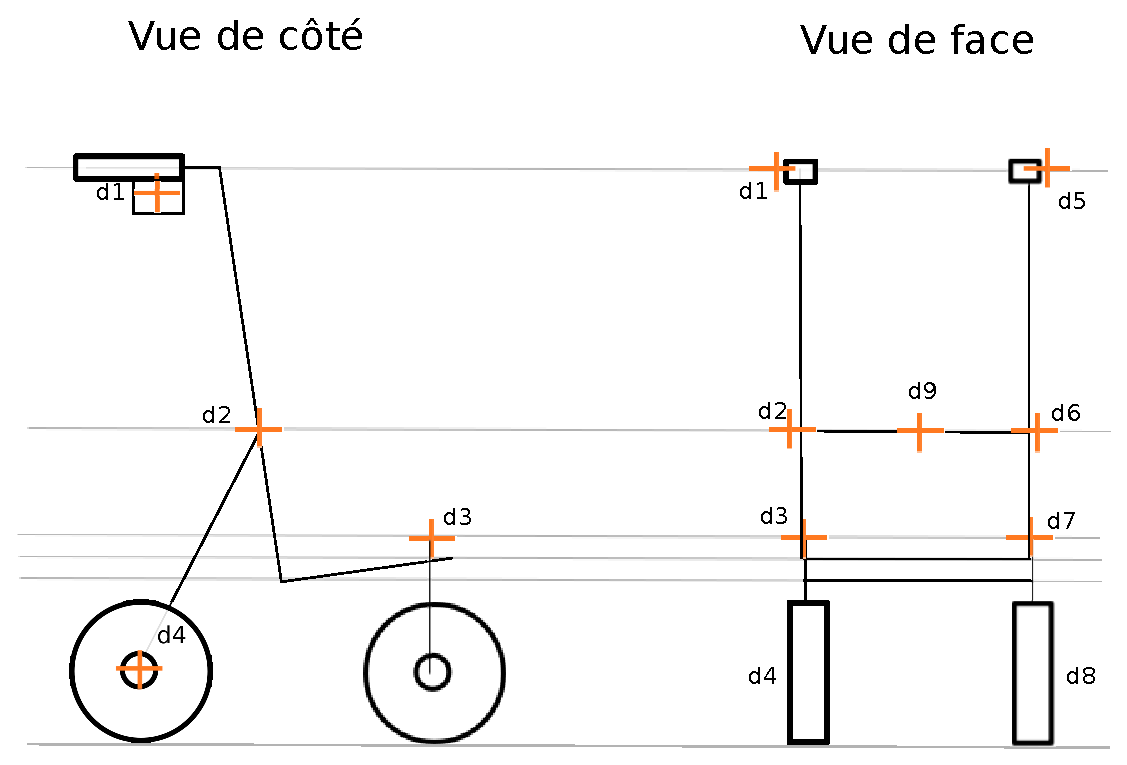
\includegraphics[width=0.7\columnwidth]{images/deambulateur.eps}
\label{fig:deambulateur}
\caption{Vue de face et vue de côté, positionnement des marqueurs sur le déambulateur.}
\end{figure}


\subsection{Equipement du déambulateur}

\subsubsection{Encodeurs}

Le déambulateur est équipé d'un encodeur sur chaque roue.
La figure \ref{fig:encodeur} présente le montage de cette encodeur. On essaye de faire des montages en pince au maximum pour éviter de modifier la structure du déambulateur.

\begin{figure}
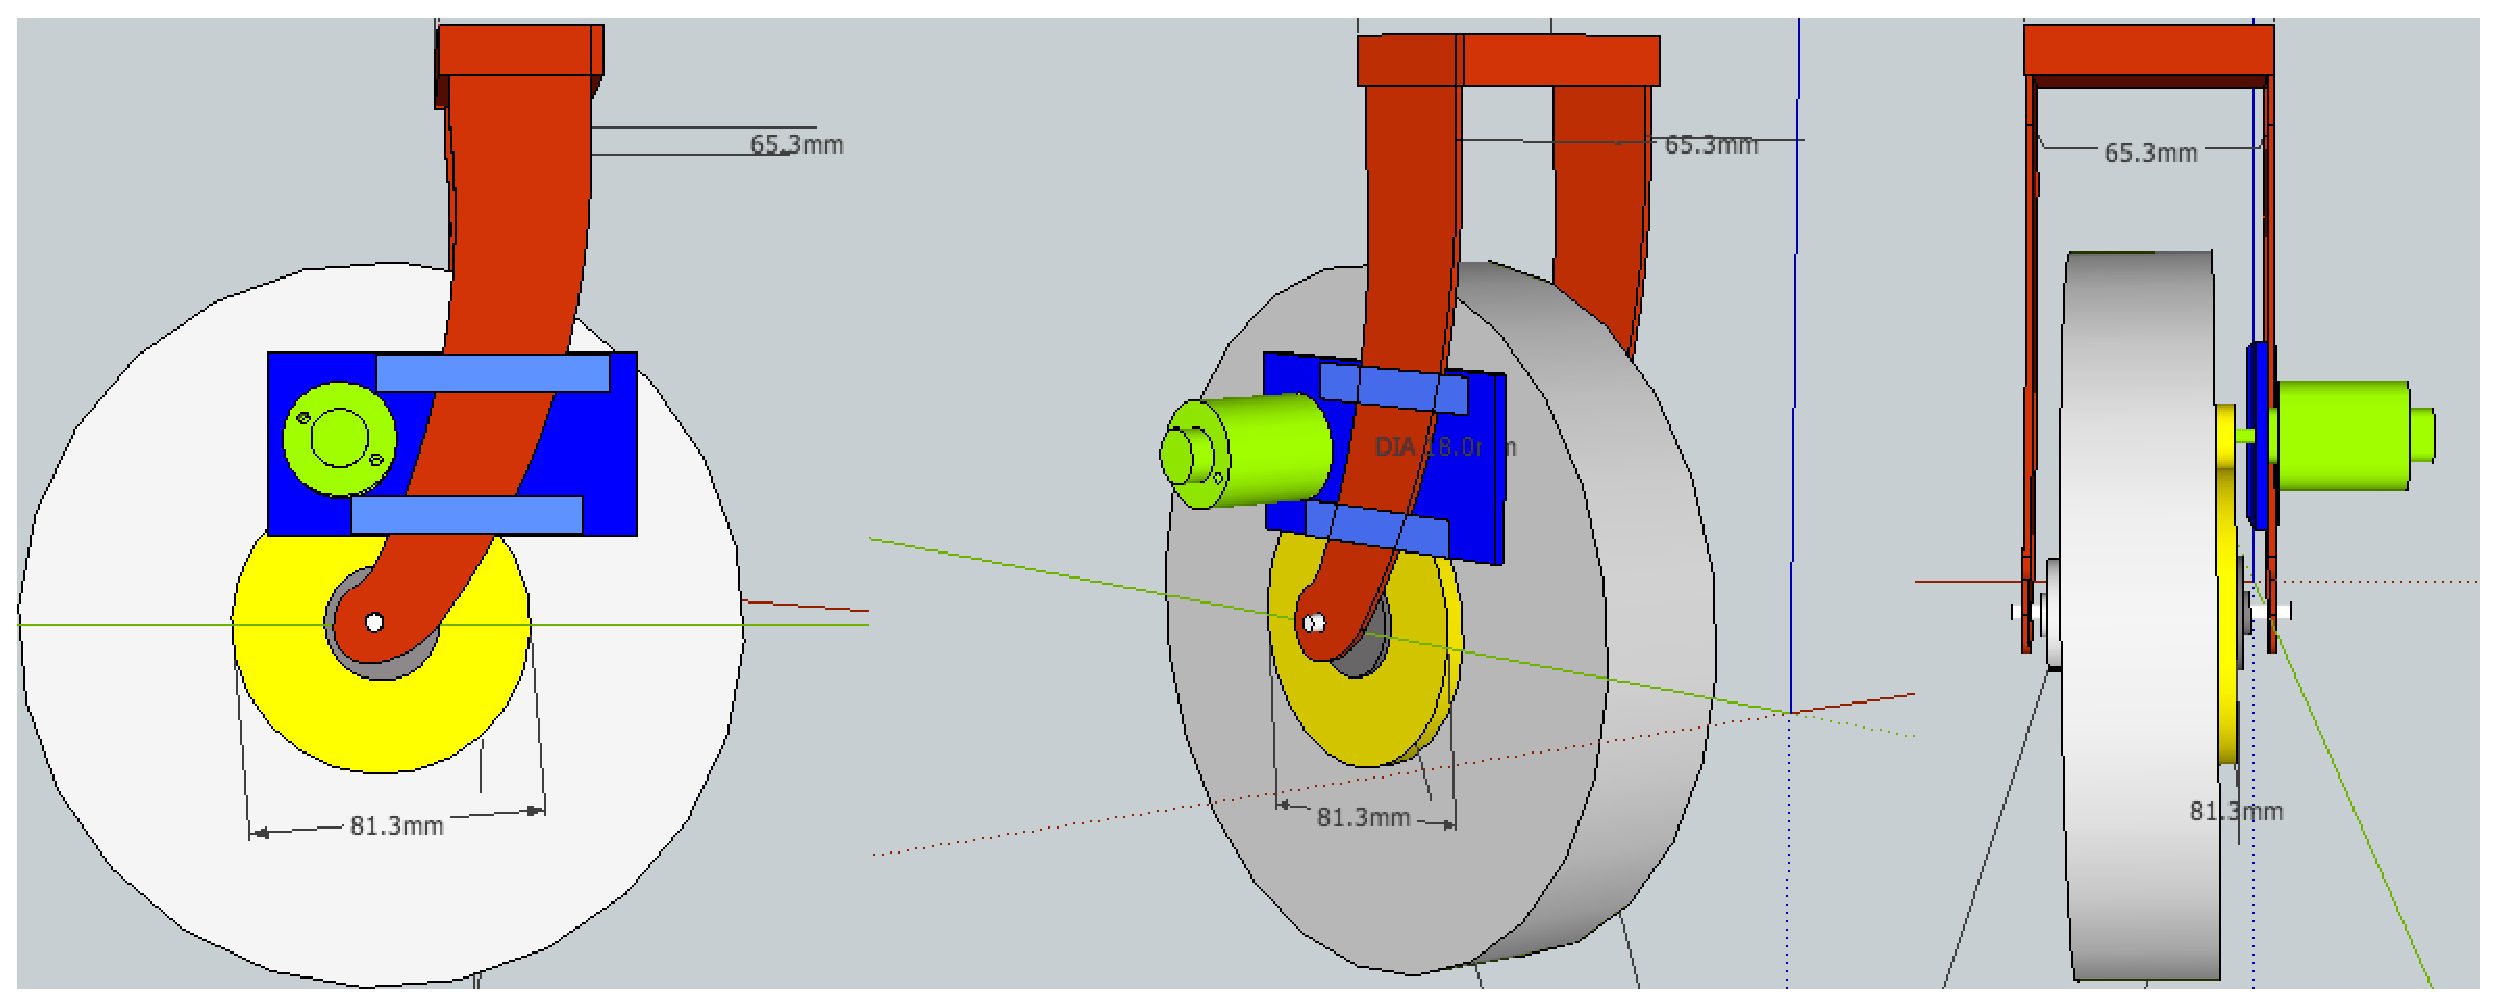
\includegraphics[width=0.8\columnwidth]{images/encodeur.eps}
\label{fig:encodeur}
\caption{Montage des encodeurs sur les roues.}
\end{figure}

\subsubsection{Gyro, accelero}

Le déambulateur est équipé d'une central inertielle avec gyro, accéléromètre et magneto.

\subsubsection{Kinect}

Une kinect est fixée sur le déambulateur pour capter la posture du sujet. Dans un premier temps, uniquement la position des pieds.

\subsubsection{Banc de stéréovision}

En plus/a la place de la kinect, un banc de stéréovision peut être monté sur le déambulateur.
Pour l'instant, le banc de stéréovision n'est pas monté.

\section{Déroulement de la manip}

\subsection{Synchronisation des horloges des ordinateurs}

\subsection{Lancement des scripts}

\subsection{Récupération des données}

TODO : Scripts, nomenclature et lieu de stockage ...


\bibliographystyle{plain} 
\bibliography{biblio}


\end{document}
